% В этом файле следует писать текст работы, разбивая его на
% разделы (section), подразделы (subsection) и, если нужно,
% главы (chapter).

% Предварительно следует указать необходимую информацию
% в файле SETUP.tex

%% В этот файл не предполагается вносить изменения

% В этом файле следует указать информацию о себе
% и выполняемой работе.

\documentclass [fontsize=14pt, paper=a4, pagesize, DIV=calc]%
{scrartcl}
% ВНИМАНИЕ! Для использования глав поменять
% scrartcl на scrreprt

% Здесь ничего не менять
\usepackage [T2A] {fontenc}   % Кириллица в PDF файле
\usepackage [utf8] {inputenc} % Кодировка текста: utf-8
\usepackage [russian] {babel} % Переносы, лигатуры

%%%%%%%%%%%%%%%%%%%%%%%%%%%%%%%%%%%%%%%%%%%%%%%%%%%%%%%%%%%%%%%%%%%%%%%%
% Создание макроса управления элементами, специфичными
% для вида работы (курс., бак., маг.)
% Здесь ничего не менять:
\usepackage{ifthen}
\newcounter{worktype}
\newcommand{\typeOfWork}[1]
{
	\setcounter{worktype}{#1}
}

% ВНИМАНИЕ!
% Укажите тип работы: 0 - курсовая, 1 - бак., 2 - маг.,
% 3 - бакалаврская с главами.
\typeOfWork{1}
% Считается, что курсовая и бак. бьются на разделы (section) и
% подразделы (subsection), а маг. — на главы (chapter), разделы и
%  подразделы. Если хочется,
% чтобы бак. была с главами (например, если она большая),
% надо выбрать опцию 3.

% Если при выборе 2 или 3 вы забудете поменять класс
% документа на scrreprt (см. выше, в самом начале),
% то получите ошибку:
% ./aux/appearance.tex:52: Package scrbase Error: unknown option ` chapterprefix=

%%%%%%%%%%%%%%%%%%%%%%%%%%%%%%%%%%%%%%%%%%%%%%%%%%%%%%%%%%%%%%%%%%%%%%%%
% Информация об авторе и работе для титульной страницы

\usepackage {titling}

% Имя автора в именительном падеже (для маг.)
\newcommand {\me}{%
Е.\,А.~Тактаров%
}

% Имя автора в родительном падеже (для курсовой и бак.)
\newcommand {\byme}{%
Е.\,А.~Тактарова%
}

% Научный руководитель
\newcommand{\supervisor}%
{к.ф.-м.н., доцент Е. М. Андреева}

% идентифицируем пол (только для курсовой и бак.)
\newcommand{\bystudent}{
Студента %Студентки % Для курсовой: с большой буквы
}

% Год публикации
\date{2019}

% Название работы
\title{Разработка системы проведения опросов аудитории\\ во время публичных выступлений}

% Кафедра
%

\newcommand {\direction} {%
Направление подготовки\\02.\ifthenelse{\value{worktype} = 2}{04}{03}.02 ---
Фундаментальная информатика\\и информационные технологии%
}

%%%%%%%%%%%%%%%%%%%%%%%%%%%%%%%%%%%%%%%%%%%%%%%%%%%%%%%%%%%%%%%%%%%%%%%%
% Другие настраиваемые элементы текста

% Листинги с исходным кодом программ: укажите язык программирования
\usepackage{listings}
\lstset{
    language=[ISO]C++,%  Язык указать здесь
    basicstyle=\small\ttfamily,
    breaklines=true,%
    showstringspaces=false%
    inputencoding=utf8x%
}
% полный список языков, поддерживаемых данным пакетом, есть,
% например, здесь (стр. 13):
% ftp://ftp.tex.ac.uk/tex-archive/macros/latex/contrib/listings/listings.pdf

\usepackage{color}
\definecolor{lightgray}{rgb}{.9,.9,.9}
\definecolor{darkgray}{rgb}{.4,.4,.4}
\definecolor{purple}{rgb}{0.65, 0.12, 0.82}
\lstdefinelanguage{JavaScript}{
	keywords={break, case, catch, continue, debugger, default, delete, do, else, false, finally, for, function, if, in, instanceof, new, null, return, switch, this, throw, true, try, typeof, var, void, while, with},
	morecomment=[l]{//},
	morecomment=[s]{/*}{*/},
	morestring=[b]',
	morestring=[b]",
	ndkeywords={class, export, boolean, throw, implements, import, this,require},
	keywordstyle=\color{blue}\bfseries,
	ndkeywordstyle=\color{cyan}\bfseries,
	identifierstyle=\color{black},
	commentstyle=\color{purple}\ttfamily,
	stringstyle=\color{red}\ttfamily,
	sensitive=true
}


\usepackage{xcolor}

\colorlet{punct}{red!60!black}
\definecolor{background}{HTML}{EEEEEE}
\definecolor{delim}{RGB}{20,105,176}
\colorlet{numb}{magenta!60!black}

\lstdefinelanguage{json}{
	basicstyle=\normalfont\ttfamily,
	numbers=left,
	numberstyle=\scriptsize,
	stepnumber=1,
	numbersep=8pt,
	showstringspaces=false,
	breaklines=true,
	frame=lines,
	backgroundcolor=\color{background},
	literate=
	*{0}{{{\color{numb}0}}}{1}
	{1}{{{\color{numb}1}}}{1}
	{2}{{{\color{numb}2}}}{1}
	{3}{{{\color{numb}3}}}{1}
	{4}{{{\color{numb}4}}}{1}
	{5}{{{\color{numb}5}}}{1}
	{6}{{{\color{numb}6}}}{1}
	{7}{{{\color{numb}7}}}{1}
	{8}{{{\color{numb}8}}}{1}
	{9}{{{\color{numb}9}}}{1}
	{:}{{{\color{punct}{:}}}}{1}
	{,}{{{\color{punct}{,}}}}{1}
	{\{}{{{\color{delim}{\{}}}}{1}
	{\}}{{{\color{delim}{\}}}}}{1}
	{[}{{{\color{delim}{[}}}}{1}
	{]}{{{\color{delim}{]}}}}{1},
}




% Нумерация списков: можно при необходимести
% изменять вид нумерации (например, добавлять правую скобку).
% По умолчанию буду списки вида:
% 1.
% 2.
% Изменять вид нумерации можно в начале нумерации:
% \begin{enumerate}[1)] (В квадратных скобках указан желаемый вид)
\usepackage[shortlabels]{enumitem}
                    \setlist[enumerate, 1]{1.}

% Гиперссылки: настройте внешний вид ссылок
\usepackage%
[pdftex,unicode,pdfborder={0 0 0},draft=false,%backref=page,
    hidelinks, % убрать, если хочется видеть ссылки: это
               % удобно в PDF файле, но не должно появиться на печати
    bookmarks=true,bookmarksnumbered=false,bookmarksopen=false]%
{hyperref}


\usepackage {amsmath}      % Больше математики
\usepackage {amssymb}
\usepackage {textcase}     % Преобразование к верхнему регистру
\usepackage {indentfirst}  % Красная строка первого абзаца в разделе

\usepackage {fancyvrb}     % Листинги: определяем своё окружение Verb
\DefineVerbatimEnvironment% с уменьшенным шрифтом
	{Verb}{Verbatim}
	{fontsize=\small}

% Вставка рисунков
\usepackage {graphicx}

% Общее оформление
% ----------------------------------------------------------------
% Настройка внешнего вида

%%% Шрифты

% если закомментировать всё — консервативная гарнитура Computer Modern
\usepackage{paratype} % профессиональные свободные шрифты
%\usepackage {droid}  % неплохие свободные шрифты от Google
%\usepackage{mathptmx}
%\usepackage {mmasym}
%\usepackage {psfonts}
%\usepackage{lmodern}
%var1: lh additions for bold concrete fonts
%\usepackage{lh-t2axccr}
%var2: the package below could be covered with fd-files
%\usepackage{lh-t2accr}
%\usepackage {pscyr}

% Геометрия текста

\usepackage{setspace}       % Межстрочный интервал
\onehalfspacing

\newlength\MyIndent
\setlength\MyIndent{1.25cm}
\setlength{\parindent}{\MyIndent} % Абзацный отступ
\frenchspacing            % Отключение лишних отступов после точек
\KOMAoptions{%
    DIV=calc,         % Пересчёт геометрии
    numbers=endperiod % точки после номеров разделов
}

                            % Консервативный вариант:
%\usepackage                % ручное задание геометрии
%[%                         % (не рекомендуется в проф. типографии)
%  margin = 2.5cm,
  %includefoot,
  %footskip = 1cm
%] %
%  {geometry}

%%% Заголовки


\ifthenelse{{\value{worktype} > 1}}{%
  \KOMAoptions{%
      headings=normal,   % размеры заголовков поменьше стандартных
      chapterprefix=true,% Печатать слово Глава
      appendixprefix=true% Печатать слово Приложение
  }
}{% Печатать слово Приложение даже если нет глав
  \newcommand*{\appendixmore}{%
    \renewcommand*{\sectionformat}{%
    \appendixname~\thesection\autodot\enskip}
    \renewcommand*{\sectionmarkformat}{%
      \appendixname~\thesection\autodot\enskip}
  }
}

% шрифт для оформления глав и названия содержания
\newcommand{\SuperFont}{\Large\sffamily\bfseries}

% Заголовок главы
\ifthenelse{\value{worktype} > 1}{%
\renewcommand{\SuperFont}{\Large\normalfont\sffamily}
\newcommand{\CentSuperFont}{\centering\SuperFont}
\usepackage{fncychap}
\ChNameVar{\SuperFont}
\ChNumVar{\CentSuperFont}
\ChTitleVar{\CentSuperFont}
\ChNameUpperCase
\ChTitleUpperCase
}

% Заголовок (под)раздела с абзацного отступа
\addtokomafont{sectioning}{\hspace{\MyIndent}}

\renewcommand*{\captionformat}{~---~}
\renewcommand*{\figureformat}{Рисунок~\thefigure}

% Плавающие листинги
\usepackage{float}
\floatstyle{ruled}
\floatname{ListingEnv}{Листинг}
\newfloat{ListingEnv}{htbp}{lol}[section]

% точка после номера листинга
\makeatletter
\renewcommand\floatc@ruled[2]{{\@fs@cfont #1.} #2\par}
\makeatother


%%% Оглавление
\usepackage{tocloft}

% шрифт и положение заголовка
\ifthenelse{\value{worktype} > 1}{%
\renewcommand{\cfttoctitlefont}{\hfil\SuperFont\MakeUppercase}
}{
\renewcommand{\cfttoctitlefont}{\hfil\SuperFont}
}

% слово Глава
\usepackage{calc}
\ifthenelse{\value{worktype} > 1}{%
\renewcommand{\cftchappresnum}{Глава }
\addtolength{\cftchapnumwidth}{\widthof{Глава }}
}

% Очищаем оформление названий старших элементов в оглавлении
\ifthenelse{\value{worktype} > 1}{%
\renewcommand{\cftchapfont}{}
\renewcommand{\cftchappagefont}{}
}{
\renewcommand{\cftsecfont}{}
\renewcommand{\cftsecpagefont}{}
}

% Точки после верхних элементов оглавления
\renewcommand{\cftsecdotsep}{\cftdotsep}
%\newcommand{\cftchapdotsep}{\cftdotsep}

\ifthenelse{\value{worktype} > 1}{%
    \renewcommand{\cftchapaftersnum}{.}
}{}
\renewcommand{\cftsecaftersnum}{.}
\renewcommand{\cftsubsecaftersnum}{.}
\renewcommand{\cftsubsubsecaftersnum}{.}

%%% Списки (enumitem)

\usepackage {enumitem}      % Списки с настройкой отступов
\setlist %
{ %
  leftmargin = \parindent, itemsep=.5ex, topsep=.4ex
} %

% По ГОСТу нумерация должны быть буквами: а, б...
%\makeatletter
%    \AddEnumerateCounter{\asbuk}{\@asbuk}{м)}
%\makeatother
%\renewcommand{\labelenumi}{\asbuk{enumi})}
%\renewcommand{\labelenumii}{\arabic{enumii})}

%%% Таблицы: выбрать более подходящие

\usepackage{booktabs} % считаются наиболее профессионально выполненными
%\usepackage{ltablex}
%\newcolumntype {L} {>{---}l}

%%% Библиография

\usepackage{csquotes}        % Оформление списка литературы
\usepackage[
  backend=biber,
  hyperref=auto,
  sorting=none, % сортировка в порядке встречаемости ссылок
  language=auto,
  citestyle=gost-numeric,
  bibstyle=gost-numeric
]{biblatex}
\addbibresource{biblio.bib} % Файл с лит.источниками

% Настройка величины отступа в списке
\ifthenelse{\value{worktype} < 2}{%
\defbibenvironment{bibliography}
  {\list
     {\printtext[labelnumberwidth]{%
    \printfield{prefixnumber}%
    \printfield{labelnumber}}}
     {\setlength{\labelwidth}{\labelnumberwidth}%
      \setlength{\leftmargin}{\labelwidth}%
      \setlength{\labelsep}{\dimexpr\MyIndent-\labelwidth\relax}% <----- default is \biblabelsep
      \addtolength{\leftmargin}{\labelsep}%
      \setlength{\itemsep}{\bibitemsep}%
      \setlength{\parsep}{\bibparsep}}%
      \renewcommand*{\makelabel}[1]{\hss##1}}
  {\endlist}
  {\item}
}{}

% ----------------------------------------------------------------
% Настройка переносов и разрывов страниц

\binoppenalty = 10000      % Запрет переносов строк в формулах
\relpenalty = 10000        %

\sloppy                    % Не выходить за границы бокса
%\tolerance = 400          % или более точно
\clubpenalty = 10000       % Запрет разрывов страниц после первой
\widowpenalty = 10000      % и перед предпоследней строкой абзаца

% ----------------------------


% Стили для окружений типа Определение, Теорема...
% Оформление теорем (ntheorem)

\usepackage [thmmarks, amsmath] {ntheorem}
\theorempreskipamount 0.6cm

\theoremstyle {plain} %
\theoremheaderfont {\normalfont \bfseries} %
\theorembodyfont {\slshape} %
\theoremsymbol {\ensuremath {_\Box}} %
\theoremseparator {:} %
\newtheorem {mystatement} {Утверждение} [section] %
\newtheorem {mylemma} {Лемма} [section] %
\newtheorem {mycorollary} {Следствие} [section] %

\theoremstyle {nonumberplain} %
\theoremseparator {.} %
\theoremsymbol {\ensuremath {_\diamondsuit}} %
\newtheorem {mydefinition} {Определение} %

\theoremstyle {plain} %
\theoremheaderfont {\normalfont \bfseries} 
\theorembodyfont {\normalfont} 
%\theoremsymbol {\ensuremath {_\Box}} %
\theoremseparator {.} %
\newtheorem {mytask} {Задача} [section]%
\renewcommand{\themytask}{\arabic{mytask}}

\theoremheaderfont {\scshape} %
\theorembodyfont {\upshape} %
\theoremstyle {nonumberplain} %
\theoremseparator {} %
\theoremsymbol {\rule {1ex} {1ex}} %
\newtheorem {myproof} {Доказательство} %

\theorembodyfont {\upshape} %
%\theoremindent 0.5cm
\theoremstyle {nonumberbreak} \theoremseparator {\\} %
\theoremsymbol {\ensuremath {\ast}} %
\newtheorem {myexample} {Пример} %
\newtheorem {myexamples} {Примеры} %

\theoremheaderfont {\itshape} %
\theorembodyfont {\upshape} %
\theoremstyle {nonumberplain} %
\theoremseparator {:} %
\theoremsymbol {\ensuremath {_\triangle}} %
\newtheorem {myremark} {Замечание} %
\theoremstyle {nonumberbreak} %
\newtheorem {myremarks} {Замечания} %


% Титульный лист
% Макросы настройки титульной страницы
% В этот файл не предполагается вносить изменения

%\usepackage {showframe}

% Вертикальные отступы на титульной странице
\newcommand{\vgap}{\vspace{16pt}}

% Помещение города и даты в нижний колонтитул
\usepackage{scrlayer}
\DeclareNewLayer[
  foot,
  foreground,
  contents={%
    \raisebox{\dp\strutbox}[\layerheight][0pt]{%
      \parbox[b]{\layerwidth}{\centering Ростов-на-Дону\\ \thedate%
       \\\mbox{}
       }}%
  }
]{titlepage.foot.fg}
\DeclareNewPageStyleByLayers{titlepage}{titlepage.foot.fg}


\AtBeginDocument %
{ %
  %
  \begin{titlepage}
  %
    \thispagestyle{titlepage}

    {\centering
    %
    \MakeTextUppercase {МИНИСТЕРСТВО ОБРАЗОВАНИЯ И НАУКИ РФ}

    \vgap

    Федеральное государственное автономное образовательное\\
    учреждение высшего образования\\
    \MakeTextUppercase {Южный федеральный университет}

    \vgap

	Институт математики, механики и компьютерных наук
    имени~И.\,И.\,Воровича

    \vgap

    \direction

    \vspace* {\fill}

    \ifthenelse{\value{worktype} = 2}{%
    \me

    \vgap}{}

    {\usefont{T2A}{PTSansCaption-TLF}{m}{n}
    \MakeTextUppercase{\thetitle}}

    \ifthenelse{\value{worktype} = 2}{%
     \vgap

    Магистерская диссертация}{}
    \ifthenelse{\value{worktype} = 0}{
     \vgap

    Курсовая работа
    }{}%
    \ifthenelse{\value{worktype} = 1 \OR \value{worktype} = 3}{
     \vgap

    Выпускная квалификационная работа\\
    на степень бакалавра
    }{}%

    \vspace {\fill}

    \begin{flushright}
    \ifthenelse{\value{worktype} = 0 \OR 
                \value{worktype} = 1 \OR
                \value{worktype} = 3}{
      \bystudent \ifthenelse{\value{worktype} = 0}{3}{4}\ курса\\
      \byme
    }{}

    \vgap

    Научный руководитель:\\
    \supervisor\\
    \ifthenelse{\value{worktype} = 2}{%
    Рецензент:\\
    ученая степень, ученое звание, должность
    И. О. Фамилия
    }{}
	\end{flushright}
\ifthenelse{\value{worktype} = 0}{
\vspace{\fill}
        \begin{flushleft}
          \begin{tabular}{cc}
            \underline{\hspace{4cm}}&\underline{\hspace{5cm}}\\
            {\small оценка (рейтинг)} & {\small  подпись руководителя}\\
          \end{tabular}
          \\[1cm]
        \end{flushleft}
}{}
\ifthenelse{\value{worktype} = 1 \OR \value{worktype} = 3}{
\vspace{\fill}
        \begin{flushleft}
Допущено к защите:\\руководитель направления ФИИТ
\underline{\hspace{4cm}}
В.\,С.\,Пилиди
        \end{flushleft}
}{}


  	\vspace {\fill}
  %Ростов-на-Дону

    %\thedate

  }\end{titlepage}
  %
  %
  \tableofcontents
  %
  \clearpage
} %


% Команды для использования в тексте работы


% макросы для начала введения и заключения
\newcommand{\Intro}{\addsec{Введение}}
\ifthenelse{\value{worktype} > 1}{%
    \renewcommand{\Intro}{\addchap{Введение}}%
}

\newcommand{\Conc}{\addsec{Заключение}}
\ifthenelse{\value{worktype} > 1}{%
    \renewcommand{\Conc}{\addchap{Заключение}}%
}

% Правильные значки для нестрогих неравенств и пустого множества
\renewcommand {\le} {\leqslant}
\renewcommand {\ge} {\geqslant}
\renewcommand {\emptyset} {\varnothing}

% N ажурное: натуральные числа
\newcommand {\N} {\ensuremath{\mathbb N}}

% значок С++ — используйте команду \cpp
\newcommand{\cpp}{%
C\nolinebreak\hspace{-.05em}%
\raisebox{.2ex}{+}\nolinebreak\hspace{-.10em}%
\raisebox{.2ex}{+}%
}

% Неразрывный дефис, который допускает перенос внутри слов,
% типа жёлто-синий: нужно писать жёлто"/синий.
\makeatletter
    \defineshorthand[russian]{"/}{\mbox{-}\bbl@allowhyphens}
\makeatother


\endinput

% Конец файла



\NewBibliographyString{langjapanese}
\NewBibliographyString{fromjapanese}

\begin{document}

\Intro
Технологии проведения публичных выступлений и презентаций затрагивают навыки ораторства и дизайн медиа-сопровождения. Методы взаимодействия с аудиторией традиционно включают в первую составляющую. Выступающий, желающий взаимодействовать со слушающими, должен уже обладать определенным опытом в работе с ними и ограничен устными средствами. Крайне редко возможно почти полностью вовлечь аудиторию в выступление, ведь лишь немногие слушатели готовы, например, задать вопрос или ответить выступающему.


Распространение телефонов и мобильного доступа в интернет, позволяет использовать эти устройства как средства взаимодействия с аудиторией. Проекты, использующие эту идею, реализовывались неоднократно, но ни один из них не закрепился как широко используемый в публичных выступлениях. В первую очередь, идея взаимодействия с публикой через телефоны реализовывалась под конкретные единичные выступления. Последующие реализации, хотя и обладают обширным функционалом, в виде  опросов, голосований и чатов, представлют собой отдельные веб-сервисы, направленные на монетизацию с пользователей. Все проекты закрыты проприетарными лицензиями и требуют от пользователей загрузки презентации на сторонний сервер.

Данная работа посвящена разработке проекта портативного веб-сервиса под свободной лицензией, который позволит проводить опросы аудитории во время публичных выступлений без привлечения сторонних сервисов. Свободная лицензия позволит любому человеку изменять и расширять возможности сервиса под свои нужды.

Задача по созданию такого проекта включает разработку как веб-интерфейса пользователя (фронтенд), так и  внутренней логики сервиса (бэкенд), которые в совокупности обеспечат динамичное отображение результатов опросов.

\section{Постановка задачи}
Решение задачи будет представлено в виде веб-сервиса, имеющего следующие отличительные функции и особенности:
\begin{itemize}
	\item Создание и проведение опросов. 
	\item Динамическое отображение результатов опроса на странице.
	\item Каждый опрос имеет короткие ссылки для голосования и просмотра результатов.
	\item Параллельное проведение нескольких опросов на одном развернутом веб-сервисе.
	\item Защита от вредоносного искажения результатов. 
	\item Двустороннее взаимодействие клиента и сервера.
	\item Открытый исходный код под свободной лицензией.
\end{itemize} 


\section{Исследование предметной области}
\subsection{Обзор существующих решений}
Как и упоминалось ранее, для опросов аудитории уже существует немалое число инструментов, однако в основой массе это закрытые решения в виде веб-сервисов:
\begin{itemize}
	\item polleverywhere.com
	\item directpoll.com
	\item sli.do
	\item ficus.io
\end{itemize}
На этих сайтах и других подобных можно бесплатно один раз провести опрос или даже презентацию, но повторные показы и дополнительные функции ограничены для пользователей, не оплативших услуги сайтов. Более того, даже оплативший пользователь ограничен средствами и функциями сайта и не может модифицировать или изменить инструмент под свои нужды и цели.

Также стоит упомянуть об инструментах опросов, не использующих только Интернет~\autocite{ombea}. Такие решения применяются в университетах США~\autocite{nea} и отличаются низкой способностью к масштабированию и высокой ценой как системы, так и индивидуальных приборов голосования.

\subsection{Обзор инструментов разработки}
При создании веб-сервиса самую важную роль занимает разработка серверной части. Так как веб-сайт должен динамически взаимодействовать с сервером, то архаичная связка из веб-сервера и CGI приложения очевидно не подойдет. Для решения данной задачи необходимо выбрать один из множества современных веб-фреймворков~\autocite{wiki}, как основу для проекта. Отметим основные необходимые для задачи черты фреймворков:
 \begin{enumerate}
 	\item легковесность
 	\item инкапсуляция веб-сервера
 	\item наличие актуального функционала( \textbf{JSON}, \textbf{AJAX}, \textbf{WebSocket})
 \end{enumerate}
Рассмотрим несколько популярных фреймворков:
 \begin{itemize}
 	\item \textbf{Django} --- фреймворк на языке Python. Хотя на нем можно реализовать необходимый нам функционал, но его врядли можно назвать легковесным. Django в первую очередь предназначен для создания больших многостраничных сайтов и сервисов, которые будет длительное время поддерживать команда разработчиков и администраторов. Наличие бесполезного для задачи функционалла негативно сказывается на времени освоения и разработки~\autocite{django}.  
 	\item \textbf{Ruby on Rails} --- фреймворк на языке Ruby. Основными минусами Ruby on Rails являются проксирование через отдельный веб-сервер и общая сложность освоения как фреймворка, так и самого языка. Стоит также отметить, что этот фреймворк сильно опирается на архитектуру модель-представление-контроллер, реализация которой усложняет задачу для небольшого приложения~\autocite{ruby}.  
 	\item \textbf{Express} --- фреймворк на языке JavaScript, запускаемый на платформе Node.js. Express инкапсулирует веб-сервер,представляя только абстракцию в виде объектов HTTP запроса и ответа, а необходимый для приложения функционал, например WebSocket и шаблонизация, добавляются через совместимые модули Node.js. Так же фреймворк не затрагивает клиентскую часть веб-приложения~\autocite{express}. Express своевременно обновляется, имеет обширную документацию и является популярным выбором среди разработчиков из-за своей простоты и понятности. Основным опасением является производительность однопоточной архитектуры Node.js, однако для небольших и средних приложений Node.js и Express показывают удовлетворительные результаты~\autocite{Kai14}.
 \end{itemize}
Таким образом, для решения рассматриваемой задачи фреймворк Express подходит идеально. Так как он не затрагивает клиентскую часть сервиса, то для нее можно использовать любой легковесный JavaScript-фреймворк для создания пользовательского интерфейса.

Также важно выбрать технологию обмена данных между сервером и клиентом. Так как в нашем случае сервер должен отправлять данные, даже когда клиент не запрашивает их явно, то данное веб-приложение по определению соотвествует модели \textbf{COMET}~\autocite{Krill07}. Рассмотрим некоторые технологии реализации \textbf{COMET} в современных веб-приложениях:

\begin{description}
	\item[Спрятанный iframe] HTML-элемент \textbf{iframe}, который подгружает <<бесконечную>> подстраницу с сервера, состоящую из элементов \textbf{script} с данными. Такой метод требует особой модификации веб-сервера, но поддерживается во всех браузерах. Достаточно сложен в реализации как на сервере, так и на клиенте. 
	\item[Подгружаемый XMLHttpRequest] Аналогично с предыдущим методом, но вместо страницы загружается AJAX-запрос.
	\item[XMLHttpRequest long polling] В этой технологии браузер отправляет AJAX-запрос, но ответ получает, только когда серверу нужно отправить данные клиенту. 
	\item[WebSocket] Отдельный протокол двустороннего соединения поверх TCP. Его реализация есть во всех современных браузерах и серверах, в том числе и для Node.js. По сравнению с другими технологиями, WebSocket отличается производительностью, скоростью передачи данных и удобством в работе.
\end{description}

Исходя из этого, для данной задачи лучше всего использовать технологию WebSocket.

Реализация современных веб-сайтов без использования фреймворков для создания интерфейса и дизайна не является актуальной задачей. Вручную описывать манипуляции с иерархической структурой HTML-страницы на чистом JavaScript крайне сложно даже для данного небольшого проекта с динамическим содержанием. Стоит отметить, что разнообразие размеров экранов мобильных устройств и персональных компьютеров также осложняет ручную верстку страницы.

Существует огромное количество фронтенд-фреймворков, вряд ли среди них можно выбрать абсолютно лучший, поэтому выбор фреймворка для маленького или среднего проектов это личное предпочтение. В проекте будет использован фреймворк Vue.js. Основными его преимуществами являются:
	\begin{description}
		\item[Реактивность] Данные связываются с интерфейсом, который изменяется автоматически, когда данные обновляются.  
		\item[Легковестность и скорость] По заявлению разработчиков, Vue.js быстрее и меньше других аналогичных фреймворков~\autocite{vue}. 
		\item[Независмость от серверной части] Хотя Vue.js может интегрироваться в сервер для улучшения производительности и работы с поисковыми системами~\autocite{vue2}, однако подключение фреймворка через HTML-тег \textbf{script} успешно работает для ненагруженных страниц.  
		
	\end{description}    
 

\section{Аспекты реализации}
\subsection{Структура проекта на Node.js}
\label{subsec:project_structuture}
Для создания основы проекта с использованием Express был использовал генератор проектов \textbf{express-generator}~\autocite{npm}. Эта утилита позволяет избавится от необходимости конфигурировать встроенный сервер и параметры фреймворка. После ее выполнения в выбранном каталоге генерируется простое, готовое для запуска веб-приложение структуры, представленной на листинге~\ref{list:express-dir}.
\begin{ListingEnv}
\dirtree{%
.1 sample-app.
.2 app.js.
.2 bin.
.3 www.
.2 package.json.
.2 public.
.3 images.
.3 javascripts.
.3 stylesheets.
.4 style.css.
.2 routes.
.3 index.js.
.3 users.js.
.2 views.
.3 error.pug.
.3 index.pug.
.3 layout.pug.
} 
\caption{Структура шаблонного проекта Express}
\label{list:express-dir}   
\end{ListingEnv}

 Разберем назначение некоторых файлов и каталогов:
 \begin{description}
 	\item[package.json] файл с указаниями для пакетного менеджера npm для Node.js. Содержит список всех пакетов, от которых зависит приложение, и точку входа для Node.js.  
 	\item[bin/www] точка входа исполняемого кода JavaScript. В нем создаются и соединяются объекты HTTP-сервера и Express-приложения. Все остальные файлы кода для Node.js являются JavaScipts-модулями, которые подключаются в \textbf{www}, либо в других модулях, уже подключенных в \textbf{www}.
 	\item[app.js] файл с настройками, касающихся конкретно работы Express. Также в нем подключаются файлы с обработчиками путей запросов.   
 	\item[public/] в настройках проекта этот каталог сконфигурирован как общедоступный для  HTTP-запросов вида GET. В нем хранятся статичные файлы для клиентской части веб-сервиса. Во время его работы эти файлы доступны по запросам вида \textbf{http://project.com/stylesheets/style.css}.
 	\item[routes/]   содержит обработчики путей запросов, поступающих в Express.
 	\item[views/]   содержит файлы шаблоны веб-страниц в формате PUG.  
 \end{description}


Такой шаблон проекта значительно упростил разработку сервиса, потому что любой написанный поверх него функционал сразу можно запустить и протестировать, а готовое файловое устройство принуждает к структурированному стилю написания кода. В конечном проекте структура каталогов приложения остается такой же, и только изменяются и добавляются в них файлы кода.      
\subsection{Использование фреймворка Express}
Разработка веб-сервиса на Express сводится к написанию обработчиков путей HTTP-запросов поступающих на сервер.
\begin{ListingEnv}[H]
\begin{lstlisting}[language=JavaScript]
router.get("/get_polled",function(req, res, next){
 let id = db.create_polling_session({
	title: "poll",
	options: [
	  { title: "option1" },
	  { title: "option2" },
	  { title: "option3" }
 ]});
 res.status(200).json({link:db.polling_sessions[id].view_link});
});
	
\end{lstlisting}
\caption{Пример функции обработчика GET-запроса}
\label{list:routing_example}
\end{ListingEnv}
В примере (листинг~\ref{list:routing_example}) для объекта \textbf{router}, который затем можно экспортировать для использовании в приложении Express, определяется поведение при поступлении GET-запроса по адресу \textbf{sample.com/get\_polled}. Для этого используется анонимная функция обратного вызова, которая исполняется каждый раз при поступлении запроса. Аргументы \textbf{req}, \textbf{res}, \textbf{next} представляют, соотвественно, объекты с данными о запросе(\textbf{REQuest}), с функциями ответа (\textbf{RESponse}) и функцию для вызова следующего подходящего обработчика пути. В примере происходит взаимодействие с моделью данных и отправка клиенту ответа с результатами взаимодействия в формате JSON.

Стоит отметить, что возможность использовать регулярные выражения и сопоставление с образцом для путей запросов, а также выстраивать цепочки из обработчиков позволило выстроить в веб-сервисе относительно сложную логику ответов на запросы. Хотя описание этой логики в исходном коде не занимает много места.  

\subsection{Использование WebSocket совместно с фреймворком Express}
Для того чтобы добавить функциональность WebSocket в приложение, используется пакетом \textbf{express-ws}~\autocite{express-ws}. Этот пакет добавляет в Express функцию для создания обработчиков путей запроса соединения по протоколу WebSocket. Чтобы добавить желаемый функционал код из пакета модифицирует прототипы класса Router внутри Express и добавляет в указанный веб-сервер обработчик запросов типа:
\begin{lstlisting}[language]
GET /api/websocket HTTP/1.1
Host: server.example.com
Upgrade: websocket
Connection: Upgrade
...
\end{lstlisting}
После этого в контексте фреймворка можно писать обработчики путей для WebSocket:
\begin{ListingEnv}[H]
	\begin{lstlisting}[language=JavaScript]
app.ws('/echo', function(ws, req) {
	ws.on('message', function(msg) {
		ws.send(msg);
	});
});
	\end{lstlisting}
	\caption{Пример функции обработчика WS-запроса}
	\label{list:ws_example}
\end{ListingEnv}
В примере (листинг~\ref{list:ws_example}), в отличие от примера в листинге~\ref{list:routing_example}, нет объекта ответа \textbf{res}, но есть объект \textbf{ws} --- асинхронно открывающийся веб-сокет, представляющий соединение между конкретным клиентом и сервером. К этому объекту уже можно привязать функции обработчики для событий изменения состояния вебсокета или получения данных. Когда состояние вебсокета изменится на \textbf{OPEN}, для объекта \textbf{ws} можно вызвать метод \textbf{send} и отправить клиенту любые данные.   

Как было сказано в подразделе~\ref{subsec:project_structuture} в шаблоне \textbf{express-generator} создание объекта HTTP-сервера и связывание его с экземпляром объекта Express происходит в файле \textbf{bin/www}, который является входной точкой исполнения кода для Node.js. Такое устройство приложения по-умолчанию не подходит для \textbf{express-ws}, которому нужно вмешаться в устройство сервера и экземпляра Express. Чтобы это исправить, необходимо внести определенные изменения в файлы \textbf{app.js} и \textbf{bin/www}.

За счет того, что \textbf{app.js} импортируется в начале \textbf{www/bin}, а значит и интерпретируется раньше чем его основной код, создание экземпляров HTTP-сервера и Express было перенесено в \textbf{app.js}. Там же происходит внедрение \textbf{express-ws}.
\begin{ListingEnv}[H]
\begin{lstlisting}[language=JavaScript]
	...
var express = require('express');
var http = require('http');
	...
var app = express();
app.server = http.createServer(app); 
var expressWS = require('express-ws')(app, app.server);
	...
module.exports = app;
\end{lstlisting}
\caption{Изменения в app.js}
\label{list:appjs-ws}
\end{ListingEnv}  
Внутри \textbf{bin/www} создание сервера заменено на обращение к ссылке на веб-сервер из экземпляра Express.
\begin{ListingEnv}[H]
\begin{lstlisting}[language=JavaScript]
var app = require('../app');
	...
var server = app.server;
server.listen(port);
server.on('error', onError);
server.on('listening', onListening);
	...
\end{lstlisting}
\caption{Изменения в bin/www}
\label{list:www-ws}
\end{ListingEnv}
Таким образом, можно воспользоваться технологией WebSocket, не нарушая структуру шаблонного приложения на фреймворке Express. 

\subsection{Проектирование и разработка модели данных}
Модель данных веб-сервиса представляет информацию о его текущем состоянии и о пользовательских данных. Обычно часть информации хранится в базе данных, отделенной от основного сервера. Такой подход удобен для масштабных проектов, где важна сохранность данных в случае неполадок или ошибок в сервисе. Однако для данного проекта интегрирование работы с базой данных будет являться только обременением, потому что в нем нет важной информации, которую нужно хранить между перезапусками.

В этом проекте используется JavaScript-объект, который содержит все другие объекты-представления данных и методы взаимодействия с ними. Этот объект и весь сопутствующий код описываются в отдельном модуле \textbf{database.js}, который экспортирует экземпляр объекта. Таким образом, код в модуле интерпретируется только один раз, и, в какой бы точке проекта не был бы импортирован объект с моделью данных, это всегда будет один и тот же экземпляр.

Прежде всего нужно было определится с тем, какие данные необходимо хранить модели и как с ними будет взаимодействовать остальная логика сервиса. Для этого был составлен список требований, которым должна отвечать модель:
 
\begin{itemize}
 \item В модели может существовать неограниченное количество параллельных сессий, которые могут перемещаться между своими опросами.
 \item Каждая сессия имеет две короткие ссылки для просмотра и участия в опросе. 
 \item Имея короткую ссылку, код должен уметь быстро переходить к данным о сессии, которой она принадлежит.
 \item Код должен быстро получать список пользователей, показывающих опрос или в нем участвующих.
 \item Пользователь может голосовать и перезагружать страницу неограниченное число раз, не вызывая подтасовку результатов.
 \item Модель должна быть устойчивой к добавлению новых видов взаимодействия пользователей с сервисом.
\end{itemize}
 
На основе этих требований была разработана следующую модель представления данных (см. листинг~\ref{list:model}). В основе реализации модели лежит использование некоторых JavaScript-объектов как словарей, где ключи это свойства объекта, например словарь сессий опроса \textbf{polling\_sessions} или словарь всех пользователей подключенных к сессии для просмотра опроса \textbf{views}. Ключи генерируются, как уникальные случайные строки. Стоить отметить, что для таких объектов нельзя определять методы или наследовать их от прототипов, потому что в JavaScript метод также является свойством, и тогда возникнут трудности, если понадобится перебрать все элементы словаря. 
 
\begin{ListingEnv}
\begin{lstlisting}[language=JavaScript]
{
 polling_sessions: {
  "aebd99ccd3": {
	views: { "6feb3f116c": {WebSocket Object} },
	slaves: { "641b151c81": {WebSocket Object} },
	password: "admin",
	view_link:"ecdd",
	slave_link:"79dd4b",
	state: {
		current_poll: 0,
		title: "poll1",
		options: [
		 { title: "option1", count: 1 },
		 { title: "option2", count: 0 },
		 { title: "option3", count: 0 }
		],
		voters: {"641b151c81": 0 }
	 },
	polls: [
		{title: "poll1",
		 options: [
		 	{ title: "option1" },
			{ title: "option2" },
			{ title: "option3" }
		 ]
		},
		{title: "poll2",
		 options: [
			{ title: "option3" },
			{ title: "option4" },
			{ title: "option5" }
		 ]
		}
	]
  }
 },
 short_links: {
	"79dd4b":{ type:"slave", session: {Session Object}},
	"ecdd":	 { type: "view", session: {Session Object}}
	}
};
\end{lstlisting}
\caption{Пример объекта модели во время работы приложения}
\label{list:model}
\end{ListingEnv}
 
 Каждый пользователей в сессии представлен лишь уникальным идентификатором, по которому доступен экземпляр WebSocket. Существует два вида пользователей: просматривающие результаты опросов и в нем участвующие. Для краткости такие пользователи будут называться \textbf{view} и \textbf{slave} соотвественно. Если пользователь перезагрузит страницу, то его экземпляр WebSocket изменится, но по идентификатору модель его распознает и обновит экземпляр. Также по идентификаторам модель отслеживает, кто и за что проголосовал в опросе, поэтому отдать два голоса невозможно. 
 
 Для объектов, которые не являются словарями, например сессии опросов \textbf{<<aebd99ccd3>>}, можно определять любые методы, инкапсулирующие взаимодействие данных и пользователей. Так, например, в файле \textbf{database.js} функция \textbf{locaс\_db.patсh\_polling\_session} добавляет к передаваемому ей экземпляру новой сессии все методы, которые меняют ее состояние. 
 
\subsection{Взаимодействие клиента и сервера через протокол WebSocket}
В клиентской части веб-приложения за работу с WebSocket отвечает статичный JavaScript-файл \textbf{ws.js}, единый как для \textbf{slave}, так и для \textbf{view} пользователей. Этот скрипт извлекает идентификатор пользователя из страницы или cookie, если он там есть, а затем открывает WebSocket-соединение по адресу:     
 \begin{Verb}
 	ws:[URL веб-сервиса]/ws/[короткая ссылка]  
 \end{Verb}

Короткая ссылка в адресе соединения позволяет серверу понять, к какой сессии принадлежит пользователь. Сразу после открытия подключения (событие \textbf{open} у объекта WebSocket), клиент отправляет свой идентификатор серверу и переходит в режим ожидания ответных сообщений, содержащих, например, состояние страницы.

\begin{ListingEnv}[H]
	\begin{lstlisting}[language=JavaScript]
var db = require('../database.js');
	...
router.ws('/ws/:shortlink',function(ws,req){
 let link = db.short_links[req.params.shortlink];
 if(!link)
  next();
 let id_type = link.type;
 let poll_session = link.session;
 let got_id = false;
 ws.on('message', function(data){
  got_id = true;
  data = JSON.parse(data);
  if(!poll_session.verify_update(data.session_id,id_type,ws))
   ws.close();
 });
 setTimeout(function(){
  if(!got_id)
   ws.close();
 },4000);
});
\end{lstlisting}
\caption{Обработчик нового WebSocket соединения, поступившего на сервер}
\label{list:poll-ws}
\end{ListingEnv}

На стороне сервера новое WebSocket соединение не сразу передается под управление модели. Как видно в листинге~\ref{list:poll-ws}, новое соединение должно пройти ряд проверок перед отправкой в модель:
   \begin{itemize}
   	\item Короткая ссылка из пути запроса должна существовать в модели.
   	\item В течение четырех секунд клиент должен прислать приемлемый JSON со своим идентификатором, иначе соединение будет закрытою.
   \end{itemize}
и в самой модели внутри функции \textbf{verify\_update}:
    \begin{itemize}
 	\item Идентификатор пользователя должен существовать в сессии.
 	\item Заявленный через короткую ссылку тип пользователя должен совпадать с типом полученного идентификатора.
 	\end{itemize}
Провал хотя бы одной проверки приводит к закрытию соединения и освобождению идентификатора. Если же проверки успешны, то объект сохраняется в сессию, и функция  \textbf{polling\_session\_object.patch\_websocket} расширяет обработчик события сообщения обработчиками \textbf{polling\_session\_object.message\_from\_slave} или \textbf{polling\_session\_object.message\_from\_view}, которые получают через аргументы не только новые данные, но идентификатор и ссылку на объект WebSocket.

Как показало тестирование и отладка приложения, оказалось очень важно удалять ненужные обработчики событий, так, например, неубранный обработчик на событие \textbf{message}, приводил к множественным вызовам  \textbf{polling\_session\_object.patch\_websocket}, которые добавляли еще больше обработчиков на один WebSocket. 

На основе этой архитектуры был выстроен простой протокол сообщений в формате JSON (см. листинг~\ref{list:message-ws}), через которые клиенты могут получать новые состояния страниц, голосовать на опросах, повыситься до владельца опроса, листать опросы и так далее.
 \begin{ListingEnv}
 	\begin{lstlisting}[language=JavaScript]
{
 "session_id": "4e643652f903975fbdd304e0115bfcb6f2a53f35",
 "type": "new_state",
 "state": {
   "title": "poll",
   "options": [
	{ "title": "option1", "count": 3 },
	{ "title": "option2", "count": 0 },
	{ "title": "option3", "count": 10 },
   ]
  }
}
 	\end{lstlisting}
 	\caption{Пример сообщения клиенту от сервера с текущим состоянием приложения}
 	\label{list:message-ws}
 \end{ListingEnv}

В случае изменения данных в модели, например \textbf{slave}-клиент проголосовал в опросе, нужно послать всем пользователям обновленные данные. Если просто вызывать функцию отправки данных всем \textbf{view}-клиентам в конце callback-функции обработки сообщения от одного \textbf{slave}-клиента, то даже при паре пользователей, непрерывно меняющих голос в опросе, сервер перестанет справляться с объемами отправляемой информации, и пользователям будет приходить запоздалая и неактуальная информация.

Чтобы решить эту проблему, был использован пакет debounce~\autocite{debounce} для Node.js. Debounce предоставляет обертку для функций, не позволяющую вызывать функцию чаще, чем в определенный промежуток времени. Вызовы, произошедшие в промежуток, откладываются в очередь и выполняются через этот промежуток.
 \begin{ListingEnv}[H]
	\begin{lstlisting}[language=JavaScript]
polling_session_object.send_state_all = debounce(function() {
 var state = { title: polling_session_object.state.title, options: polling_session_object.state.options };
 for (var id in polling_session_object.views) {
		...
 view.send(JSON.stringify({ session_id: id, type: "new_state", state: state }));
  }
 for (var id in polling_session_object.slaves) {
		...
 view.send(JSON.stringify({ session_id: id, type: "new_state", state: state }));
 }
 this.send_state_all.clear();
},200);
\end{lstlisting}
\caption{Использование debounce для контроля отправки нового состояния всем пользователям}
\label{list:debounce-exmpl}
\end{ListingEnv}      

Также важно очищать очередь вызовов после отработки кода через \textbf{debounce.clear} как в примере на листинге~\ref{list:debounce-exmpl}. Тогда нескольким вызовам обернутой функции, произошедшим в один промежуток, соответствуют только один вызов целевой функции.

\subsection{Создание пользовательского интерфейса}
В данном веб-сервисе существует два основных вида страниц, которые были реализованы в первую очередь. Страница просмотра результатов опроса и страница голосования, которые в модели данных представляются \textbf{view} и \textbf{slave} пользователями соответственно(см. рисунки~\ref{fig:view} и~\ref{fig:slave} ).
 \begin{figure}[H]
	\centering
	%Здесь могла быть ваша лягушка.
	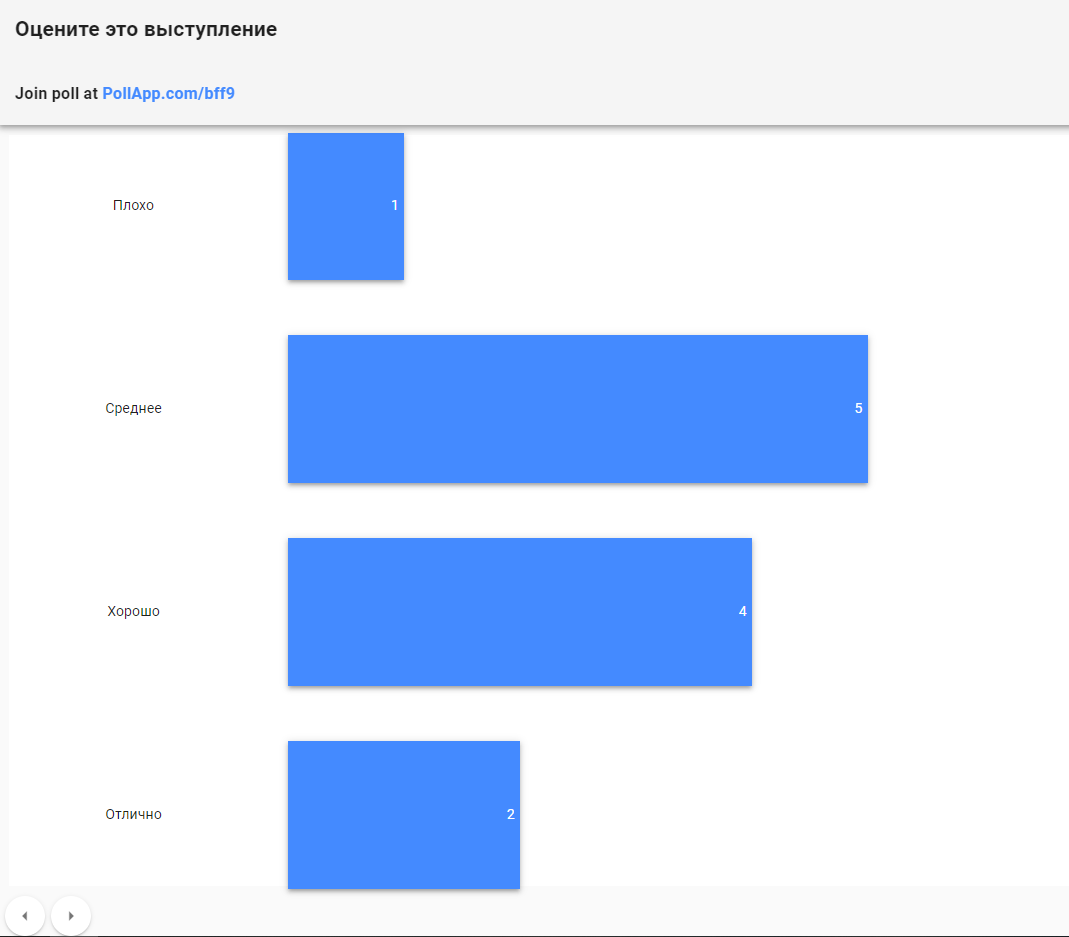
\includegraphics[scale=0.5]{img/view.PNG}
	\caption{\label{fig:view} Страница просмотра результатов опроса}
\end{figure}

\begin{figure}[H]
	\centering
	%Здесь могла быть ваша лягушка.
	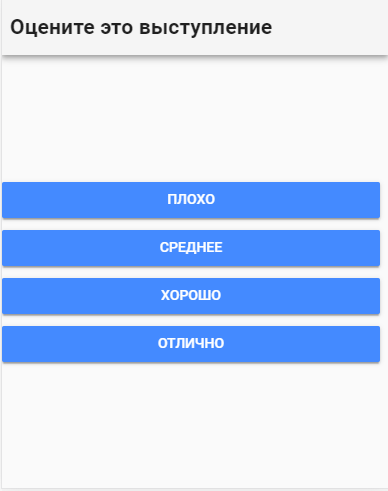
\includegraphics[scale=0.8]{img/slave.PNG}
	\caption{\label{fig:slave} Страница голосования на мобильном устройстве}
\end{figure}
Страница просмотра результатов не только динамично обновляет результаты опроса, но также показывает ссылку по которой можно присоединится к нему и, при вводе секретной фразы, указанной при создании опроса, дает пользователю контроль над проведением опроса.

Для того что бы отправлять страницы пользователям, был использован шаблонный движок Pug. Его синтаксис состоит из смеси JavaScript и видоизмененного HTML (см. листинг~\ref{list:pug-lay}). C помощью табуляции описывается древовидная структура страницы, точка обозначает блок сплошного текста, а \textbf{<<\#{...}>>} окружает JavaScript-код, который интерпретируется на стороне сервера, а результат записывает на его место~\autocite{pug}. Pug --- мощный инструмент шаблонизации, но в данном проекте он используется, чтобы передать пользователю только основу страницы, в которой указаны ссылки на загрузку частей фреймворка и начальные данные о состоянии страницы.
 \begin{ListingEnv}
	\begin{lstlisting}[language=pug]
doctype html
html
 head
  meta(charset="utf-8")
  script(src="/javascripts/js.cookie.js")
  link(rel="stylesheet" href="https://unpkg.com/vue-material@beta/dist/vue-material.min.css")    
 body
  script(type='text/javascript').
  \end{lstlisting}
  \begin{lstlisting}[language=JavaScript]
     var sessionInfo = {
	 	id : "#{session_id}",
	 	type : "#{session_type}",
		viewLink: "#{view_shortlink}",
		slaveLink:  "#{slave_shortlink}"
	}  
\end{lstlisting}
\begin{lstlisting}[language=pug]
  main#app 
	block content
  script(src="/javascripts/ws.js")
  script(src="https://cdn.jsdelivr.net/npm/vue/dist/vue.js")
  script(src="https://unpkg.com/vue-material@beta")
  script.
	Vue.use(VueMaterial.default);
  block footer_scripts
	\end{lstlisting}
	\caption{Шаблон разметки страницы на языке Pug}
	\label{list:pug-lay}
\end{ListingEnv}      

Основную работу по отображению элементов выполняет фреймворк Vue.js. Ядро фреймворка загружается на страницу из CDN (пер. Сеть доставки содержимого) через тег \textbf{script}. После этого в последующих скриптах можно описывать компоненты страницы как объекты Vue. 

В файлах \textbf{javascripts/slave\_ui.js} и \textbf{javascripts/view\_ui.js} определены Vue-компоненты для соответствующих страниц. Компоненты напрямую связаны с данными, например, о состоянии страницы, и если изменяются данные, то компоненты перерисовываются. Синтаксис шаблонов Vue позволяет описывать элементы через условия и циклы, что и используется, чтобы отображать опросы с любым количеством вариантов.

В файле \textbf{javascripts/ws.js} описана логика соединения с сервером через WebSocket, но ее запуск обернут в метод  
\textbf{sessionInfo.init\_WS}. Это связано с тем, что экземпляру Vue требуется время, чтобы полностью создаться и связать данные с компонентами, поэтому вызов \textbf{init\_WS} происходит только после события \textbf{created} в экземпляре Vue. Тогда фреймворк уже отслеживает изменения данных.
 
Для других страниц нет необходимости в функционале WebSocket. Чтобы отправить данные с созданным опросом достаточно упаковать их в формат JSON и отправить через POST-запрос на сервер. Данные о опросах на сервере доступны в формате JSON по GET-запросу. Если  отправленные данные не соответствуют требованиям сервера, то в ответе на запрос содержится текст ошибки, которые на стороне клиента показывается как всплывающее предупреждение.        

\newpage
\section{Обзор проекта}
\subsection{Внутреннее устройство}
За время разработки общая структура проекта не менялась кардинально, JavaScript-модули и другие файлы кода, реализующий новый функционал, добавлялись в соответствующие каталоги. В текущей итерации разработки проект имеет структуру, представленную на листинге~\ref{list:poll-dir}. Некоторые из новых файлов уже упоминались выше, но все же разберем каждый из них:

\begin{ListingEnv}[p]
\dirtree{%
	.1 poll\_app.
	.2 bin.
	.3 www.
	.2 public.
	.3 images.
	.3 javascripts.
	.4 builder\_ui.js.
	.4 index\_ui.js.
	.4 slave\_ui.js.
	.4 view\_ui.js.
	.4 js.cookie.js.
	.4 ws.js.
	.3 stylesheets.
	.4 builder\_style.css.
	.4 index\_style.css.
	.4 slave\_style.css.
	.4 view\_style.css.
	.2 routes.
	.3 poll.js.
	.2 views.
	.3 error.pug.
	.3 index.pug.
	.3 layout.pug.
	.3 builder.pug.
	.3 view.pug.
	.3 slave.pug.
	.2 app.js.
	.2 database.js.
	.2 package.json.
	.2 LICENSE.
	.2 README.md.
}
\caption{Структура проекта Poll\_app}
\label{list:poll-dir}
\end{ListingEnv}
\begin{description}
	\item[javascripts/\dots\_ui.js] Это JavaScript-файлы, в которых содержится описание интерфейса каждой страницы в контексте фреймворка Vue.js. 
	\item[javascripts/ws.js] В этом файле описана логика соединения клиента и сервера по протоколу WebSocket.
	\item[javascripts/js.cookie.js] Свободная легковесная библиотека для работы с куки на стороне клиента.
	\item[stylesheets/\dots\_style.css] Каскадные таблицы стилей для каждой страницы.
	\item[views/ \dots\space.pug] Файлы HTML-шаблонов страниц в формате Pug. Каждый шаблон подключает файл \textbf{layout.pug}, в котором описаны общие для всех страниц HTML-элементы. 
	\item[routes/poll.js] Файл, в котором описаны все пути HTTP-запросов, поступающих в приложение, и их обработчики в контексте фреймворка Express.
	\item[database.js] JavaScript-модуль, экспортирующий экземпляр объекта модели данных в приложении.  
\end{description}

Развернутое приложение состоит из двух вспомогательных статичных веб-страниц и из двух уже упомянутых динамичных веб-страниц участия и просмотра опроса, уникальных для каждой отдельной сессии.  По адресам <<\textbf{/}>> и <<\textbf{/index}>>, доступна начальная страница(см. рисунок ~\ref{fig:index}). На ней отображаются все текущие и доступные сессии опросов. К текущим сессиям можно присоединиться как зритель или участник. А доступные опросы можно начать, если ввести кодовое слово, с которым опрос был создан.

\begin{figure}[H]
	\centering
	%Здесь могла быть ваша лягушка.
	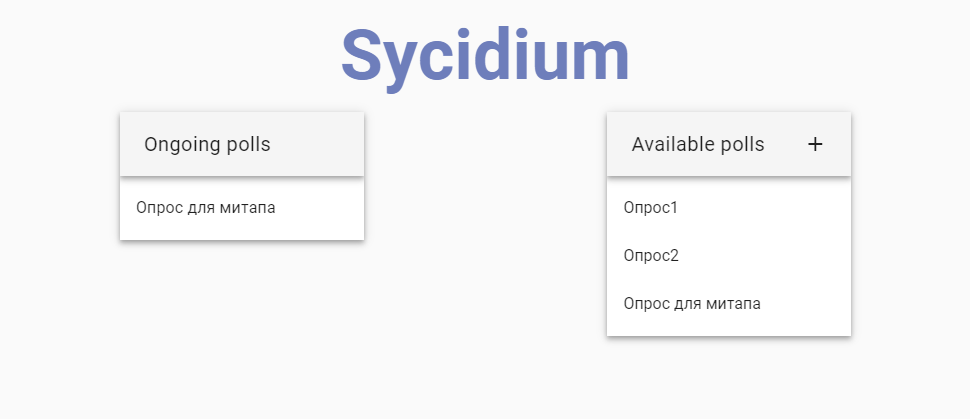
\includegraphics[width=\textwidth]{img/index.PNG}
	\caption{\label{fig:index} Начальная страница веб-сервиса}
\end{figure}

Страница по адресу <<\textbf{/build\_poll}>>(см. рисунок~\ref{fig:builder}), позволяет добавить на сервер заготовку сессии опросов. В динамичном интерфейсе, реализованном с помощью Vue.js, пользователь может добавить произвольное количество опросов и их вариантов в них, указать пароль и название сессии.

 \begin{figure}[H]
 	\centering
 	%Здесь могла быть ваша лягушка.
 	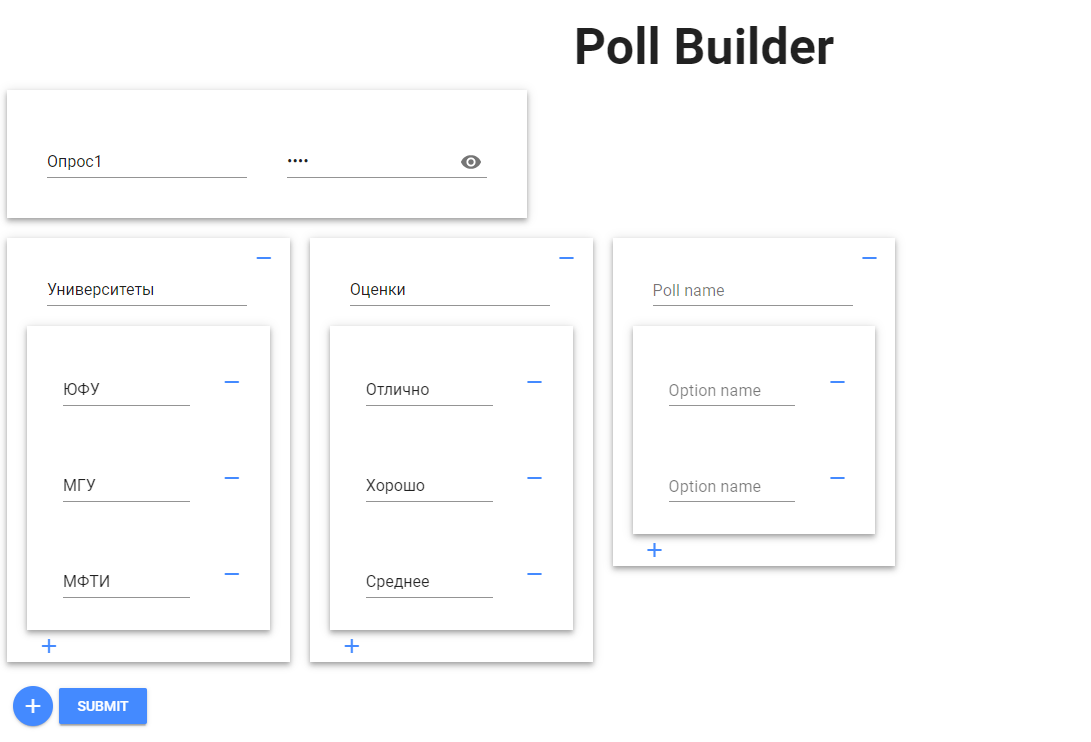
\includegraphics[width=\textwidth]{img/builder.PNG}
 	\caption{\label{fig:builder} Страница создания опроса}
 \end{figure}
 
  
Страницы просмотра и участия в опросе имеют уникальные для каждого опроса короткие ссылки. Страница участия оптимизирована в первую очередь для мобильных устройств. Со страницы просмотра можно управлять ходом опроса, если ввести кодовое слово. Содержание этих страниц обновляется динамически, когда изменяется состояние опроса.     
          
\subsection{Установка и использование проекта}  
Исходные коды проекта можно получить в Git репозитории по ссылке:
\href{https://github.com/Jeday/Sycidium.git}{github.com/Jeday/Sycidium.git}

Для GNU/Linux систем:
\begin{enumerate}
	\item Установите последние версии Node.js и npm.
	\item Склонируйте файлы приложения в отдельную папку.
	\item В корне приложения выполните \textbf{npm install}, чтобы установить зависимости.
	\item Запустите приложение через \textbf{npm start}.
	\item Приложение доступно по адресу \textbf{http://localhost:3000/}
\end{enumerate}

Чтобы запусть приложение в рабочем режиме с произвольным портом нужно изменить порт в файле \textbf{package.json} и выполнить \textbf{npm run prod}.
  \begin{ListingEnv}
 \begin{lstlisting}[language=JavaScript]
{
 "name": "poll-app",
 "version": "0.7.0",
 "private": true,
 "scripts": {
 	"start": "node ./bin/www",
 	"prod": "NODE_ENV=production PORT=80 node ./bin/www"
    },
 "dependencies": {
	...
 }
}

\end{lstlisting}
	\caption{Файл package.json с установленным портом 80}
\label{list:pack-json}
\end{ListingEnv}      



\newpage
\Conc
В рамках данной работы был реализован полноценный веб-сервис для проведения опросов во время публичных выступлений. Все поставленные задачи выполнены и цели достигнуты:
\begin{itemize}
	\item Веб-сервис позволяет параллельно создавать, запускать и управлять неограниченным количеством опросов.
	\item Пользователи могут сразу же поучаствовать в опросе со своего мобильного устройства, перейдя по короткой ссылке, указанной на экране опроса.
	\item Результаты голосования отображаются динамически на странице просмотра результатов.
	\item Реализована основная защита от вредоносного вмешательства в процесс опроса, не позволяющая испортить результаты или остановить ход опроса.
	\item Веб-сервис имеет открытые исходные коды на сайте \textbf{GitHub.com} и доступен для развертывания, использования и модификации по свободной лицензии MIT. 
\end{itemize}              
Наиболее очевидным способом улучшения сервиса является добавление других возможностей для взаимодействия с аудиторией и интеграцией с потоком презентации. К таким функциям можно отнести: чат, отображающийся на экране; слияние опросов и слайдом презентации; разные формы и виды опросов.


\newpage
% Печать списка литературы (библиографии)
\printbibliography[%{}
    heading=bibintoc%
    %,title=Библиография % если хочется это слово
]
% Файл со списком литературы: biblio.bib
% Подробно по оформлению библиографии:
% см. документацию к пакету biblatex-gost
% http://ctan.mirrorcatalogs.com/macros/latex/exptl/biblatex-contrib/biblatex-gost/doc/biblatex-gost.pdf
% и огромное количество примеров там же:
% http://mirror.macomnet.net/pub/CTAN/macros/latex/contrib/biblatex-contrib/biblatex-gost/doc/biblatex-gost-examples.pdf

\appendix
\ifthenelse{\value{worktype} > 1}{%
  \addtocontents{toc}{%
      \protect\renewcommand{\protect\cftchappresnum}{\appendixname\space}%
      \protect\addtolength{\protect\cftchapnumwidth}{\widthof{\appendixname\space{}} - \widthof{Глава }}%
  }%
}{
  \addtocontents{toc}{%
      \protect\renewcommand{\protect\cftsecpresnum}{\appendixname\space}%
      \protect\addtolength{\protect\cftsecnumwidth}{\widthof{\appendixname\space{}}}%
  }%
}


\end{document}
